\documentclass[9pt,twocolumn,twoside]{../../styles/osajnl}
\usepackage{fancyvrb}

\journal{i524} 

\title{H-Store}

\author[1,*,+]{Karthick Venkatesan}


\affil[1]{School of Informatics and Computing, Bloomington, IN 47408, U.S.A.}


\affil[*]{Corresponding authors: vkarthickprabu@gmail.com}

\affil[+]{HID - S17-IO-3023}

\dates{paper1, \today}

\ociscodes{H-Store,OLTP, I524}

% replace this with your url in github/gitlab
\doi{\url{https://github.com/cloudmesh/sp17-i524/tree/master/paper1/S17-IO-3023/report.pdf}}


\begin{abstract}
"NewSQL" denotes a class of modern (RDBMS)relational database management systems that seek to provide the same scalable performance of NoSQL systems for online transaction processing (OLTP) read-write workloads while still maintaining the ACID 
guarantees of a traditional database system. H-Store is one the first 
NewSQL system which is a complete redesign of the traditional RDMS database.
\end{abstract}

\setboolean{displaycopyright}{true}

\begin{document}

\maketitle

\section{Introduction}

H-Store is an experimental database management system (DBMS) designed for 
online transaction processing applications 
that was developed by a team of researchers  at Brown University, Carnegie 
Mellon University, the Massachusetts Institute of Technology, and Yale 
University.

Traditional SQL databases offer rich transaction capabilities, ad-hoc query and reporting capability, and vast amounts of standards-based tooling. Where they 
fall short is in the ability to scale out to meet the needs of modern, 
high-performance applications.NoSQL Databases are a solution to issues of scale that 
emerged as organizations began dealing with immense volumes, velocity, and 
variety of big data from a multitude of sources. NoSQL solutions offered 
availability, flexibility and scale. However, they came with difficult 
tradeoffs - sacrifice of data consistency and transactional (ACID) guarantees, 
loss of ad-hoc query capability and increased application complexity.By 
removing just the parts of SQL that hampered scalability and performance, it 
was able to increase both while maintaining key advantages of SQL 
systems.NewSQL technologies offer the best of both worlds: the scale of NoSQL 
with the ACID guarantees, strong consistency, minimized application complexity 
and interactivity of SQL. The H-Store DBMS belongs to this class of parallel 
database management systems, called NewSQL.

The current RDBMS systems were architected 
more than 25 years ago, when
hardware characteristics were much different than today.
Today processors are thousands of times faster and memories are
thousands of times larger. Disk volumes have increased
enormously, making it possible to keep essentially everything, if
one chooses to in memory \cite{stonebraker2007}. The current day DBMS 
include the following architectural features which are not fully utilising 
the technological advancements in the last 25 years  .
\begin{itemize}
\renewcommand{\labelitemi}{\scriptsize$\bullet$} 
\item Disk oriented storage and indexing structures
\item Multithreading to hide latency
\item Locking-based concurrency control mechanisms
\item Log-based recovery
\end{itemize}

H-Store is a complete redesign of the traditional RDMS database designed to fully leverage the advancements in hardware capabilities over the last 25 years and 
experimetal results show that the OLTP processing on a H-Store database is 
faster 
by a factor of 82 \cite{stonebraker2007}.

\section{System Architecture}

\begin{figure}[http]
\centering
\graphicspath{ {images/} }
\fbox{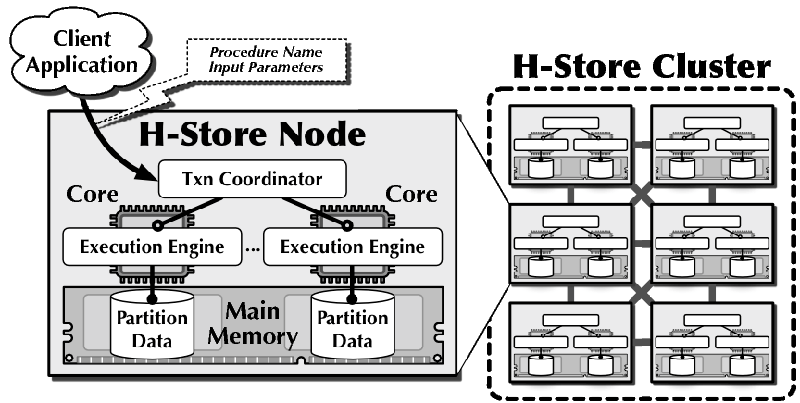
\includegraphics[width=\linewidth]{hstore}}
\caption{H-Store Architecture} \cite{www-H-StoreArch}
\label{fig:false-color}
\end{figure}

A single H-Store instance as in Figure 1 consists of a cluster 
of two or more computational nodes deployed within the same domain \cite{www-H-StoreArch}. 
\begin{itemize}
\item A node is a single physical computer system that hosts one or more execution sites and one transaction coordinator. 
\item A site is the logical operational entity in the system; it is a single-threaded 
execution engine that manages some portion of the database and is responsible 
for executing transactions on behalf of its transaction coordinator. 
\item The transaction coordinator is responsible for ensuring the serializability of 
transactions along with the coordinators located at other nodes.
\item A typical H-Store node contains one or more multi-core CPUs, each with multiple hardware 
threads per core. As such, multiple sites are assigned to nodes independently 
and do not share any data structures or memory.
\end{itemize}

\section{Storage Architecture}

Every table in H-Store is horizontally divided into multiple shards that each 
consist of a disjoint sub-section of the entire table. The boundaries of a 
table’s fragments are based on the selection of a  column for that table; 
each tuple is assigned to a fragment based on the hash values of this 
attribute. H-Store also supports partitioning tables on multiple columns. 
Related fragments from multiple tables are combined together into a partition 
that is distinct from all other partitions. Each partition is assigned to 
exactly one site.

All tuples in H-Store are stored in main memory on each node; the system never 
needs to access a disk in order to execute a query.It replicates partitions to 
ensure both data durability and availability in the event of a node failure. 
Data replication in H-Store occurs in two ways: (1) replicating partitions on 
multiple nodes and (2) replicating an entire table in all partitions. For the 
former, H-Store adopts the k-safety concept, where $k$ is defined by the 
administrator as the number of node failures a database can tolerate before it 
is deemed unavailable \cite{www-H-StoreArch}.

\section{Transaction Processing}

Client applications make calls to the H-Store system to execute pre-defined 
stored procedures. Each procedure is identified by a unique name and consists 
of user-written Java control code intermixed with parameterized SQL commands. 
The input parameters to the stored procedure can be scalar or array values, and queries can be executed multiple times.

Each instance of a stored procedure executing in response to a client request 
is called a transaction. Similarly as with tables, stored procedures in H-Store are assigned a partitioning attribute of one or more input parameters. When a 
new request arrives at a node, the transaction coordinator hashes the value of 
the procedure’s partitioning parameter and routes the transaction request to 
the site with the same id as the hash. Once the request arrives at the proper 
site, the system invokes the procedure’s Java control code, which will use 
the H-Store API to queue one or more queries in a batch. The control code 
invokes another command in H-Store to block the transaction while the execution engine executes the batched queries.

All of operations within a transaction are atomic across all the partitions 
involved in the transaction. When a transaction executes, it has exclusive 
access to the data at the partitions that it locks, therefore all of its 
operations execute on a consistent view of the database and are isolated from 
all other transactions (since no other transactions execute concurrently at 
those partitions). Finally, with snapshots and command logging, the state of 
the database is completely recoverable and all changes made by transactions are durable \cite{www-H-StoreArch} .

\section{Documentation}

\begin{itemize}
\renewcommand{\labelitemi}{\scriptsize$\bullet$} 
\item Detailed documentation on H-Store  Deployment , Configuration,Debugging 
and Development is available at  \cite{www-H-Store}
\item H-Store DBMS is open source and complete source code is available in the  
\cite{github-H-Store} github repository. 
\end{itemize}

\section{Commercial Use}

A commercial implementation of H-Store is VoltDB. VoltDB was developed for 
production environments, and thus it is focused on high-performance throughput 
for single-partition transactions and provides robust handling of failures that are needed for a main memory system.H-Store uses VoltDB’s VoltProcedure API, so any stored procedures written for VoltDB work work in H-Store 
\cite{www-H-StoreFaq}. 

\section{Related Technologies-Other In Memory New SQL databases}

\begin{itemize}
\item \textbf{VoltDB}:VoltDB is an in-memory, scale-out SQL database purpose-built to power a new
generation of applications that thrive on fast, smart data. Tapping the lightning
speed and real-time analytics of VoltDB, organizations are able to add context
and intelligence to data – the instant it arrives – to make real-time transactional
decisions that maximize business value \cite{www-VoltDB}.

\item \textbf{Clustrix}:Clustrix provides the leading scale-out SQL database engineered for the cloud
and the database built specially to meet the unique growth, performance and
availability demands of today’s e-commerce sites. ClustrixDB, helps to build
business critical applications that support massive transactional volume and realtime
reporting of business performance metrics. ClustrixDB delivers more than
one trillion transactions per month for customers \cite{www-ClustrixDB}.

\item \textbf{NuoDB}:NuoDB is a scale-out SQL database for the cloud and the modern datacenter. It is
the NewSQL solution designed to meet the needs of cloud-scale apps and over
50 billion connected devices in use worldwide \cite{www-NuoDB}.

\item \textbf{MemSQL}:MemSQL is a leader in real-time databases for transactions and analytics.As a
purpose built database for instant access to real-time and historical data,
MemSQL uses a familiar SQL interface and a horizontally scalable distributed
architecture that runs on commodity hardware or in the cloud \cite{www-Memsql}.
\end{itemize}

\section{Comparison of New SQL databases}

A comparison of other NewSQL  database features with H-Store is provided in Fig 2.
\begin{figure*}[]
\centering
\graphicspath{ {images/} }
\fbox{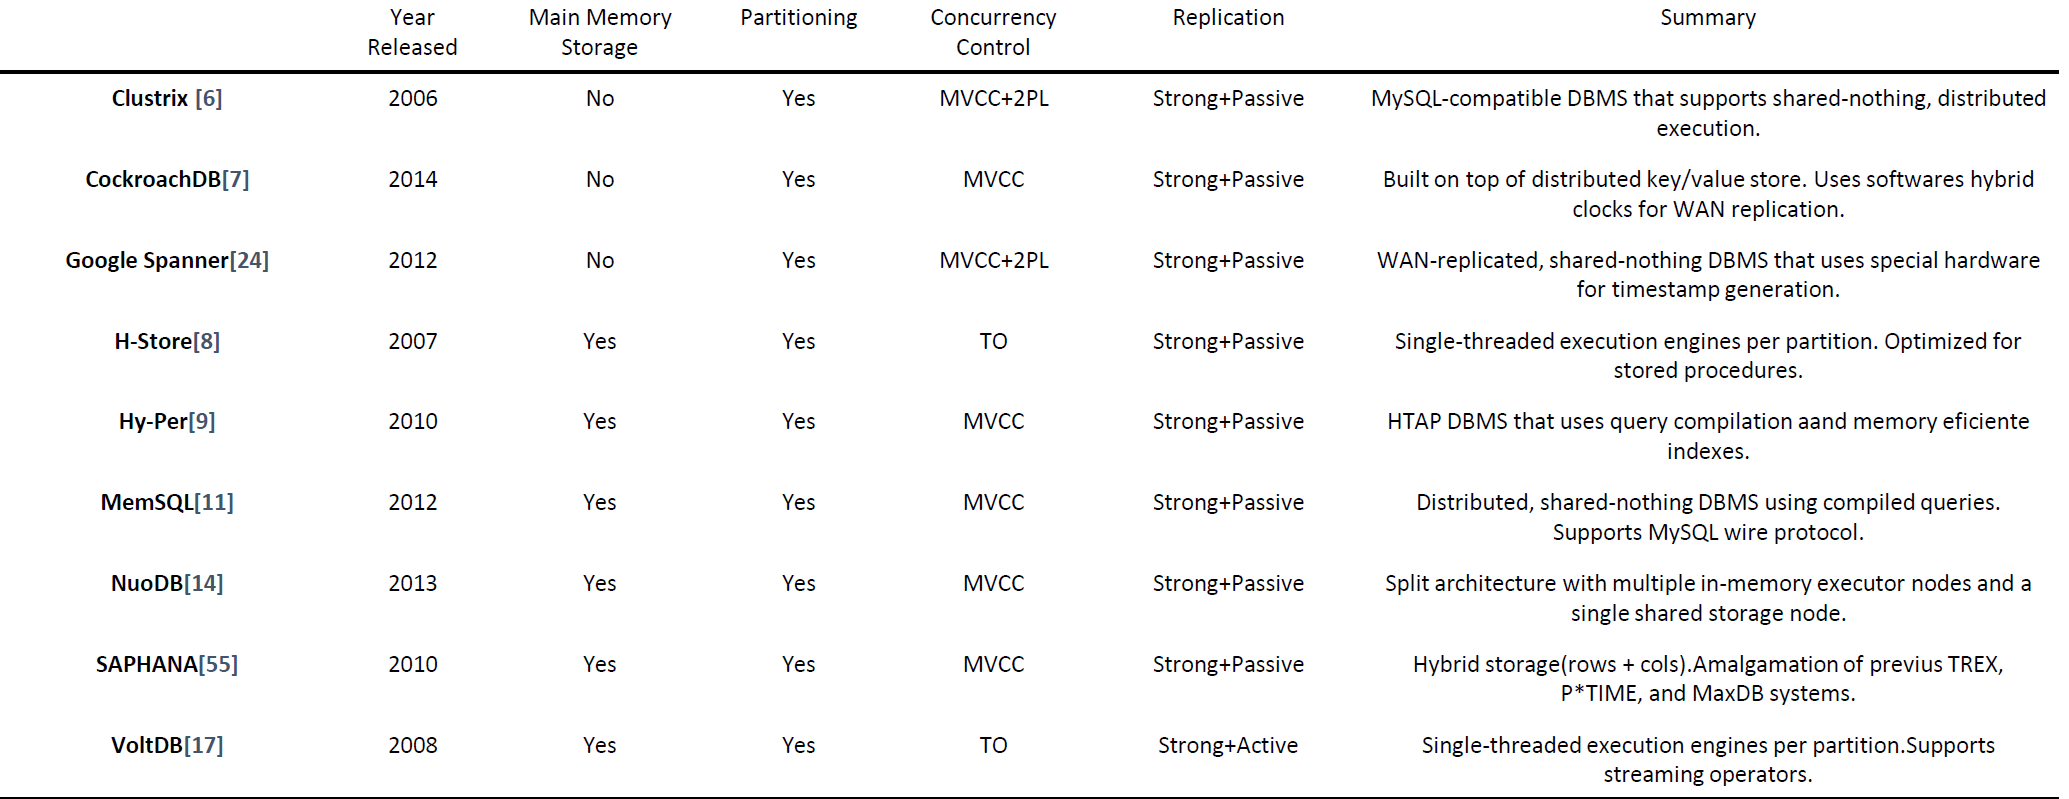
\includegraphics[width=\linewidth,height=6cm]{Compare}}
\caption{NewSQL DB Comparison} \cite{pavlo16}
\label{fig:false-color}
\end{figure*}


\section{Use Case}
 
 In Memory NewSQL databases such as H-Store are ideally suited for handling uses cases related to Fast Data \cite{www-FastData}.
\begin{itemize}
\renewcommand{\labelitemi}{\scriptsize$\bullet$} 
\item Real-time recommendation engines or hyper-personalization applications 
that can detect and act on individual customer needs in real-time.Emagine International  is a innovative company provides a real-time, adaptive contextual marketing platform and managed marketing services for mobile service providers. 
To differentiate its offering and help operators take advantage of real-time analytics and
decisioning, Emagine implemented H-Store's Commercial implementation VoltDB as the core of its
Emagine Real-time Event Decisioning (ERED) platform. This has allowed Emagine to architect
a fast data solution that requires 3 milliseconds for the ingest-analyze-decide journey through
the ERED platform, enabling Emagine to deliver customized offers to subscribers in fewer than
250 milliseconds. Mobile operators that use the ERED platform achieved a measurable ROI
in real-time personalization \cite{www-Emagine}. 

\item Real-time, "down to the last dollar" resource management applications.
More than 150,000 apps and the world’s leading advertisers rely on Airpush a mobile advertising 
company 
to deliver the industry’s highest performance, driven by exceptional ad formats
and targeting technology.The company originally built a MySQL infrastructure
to manage advertising transactions. Airpush’s
business grew exponentially, pushing the limits of
MySQL. To ensure the system would be able to
process transactions fast enough to align advertising
purchases with customer budgets, Airpush began to
look into alternative. Airpush selected VoltDB (H-Store commercial implementation),
which offerered the performance
of in-memory, the scalability of NoSQL, and the
transactional consistency of traditional relational
databases.
With VoltDB, Airpush built a  transactional, database oriented
applications against data feeds that were
previously limited to stream processing methods
because of scale. Supporting hundreds of thousands of concurrent
connections with round-trip latencies in milliseconds,
VoltDB is an ideal platform for high-speed policy
enforcement, authorization, rule evaluation, and quota
management \cite{www-Airpush}.

\end{itemize}

\section{Conclusion}
H-Store and its commercial implementation VoltDB are main memory DBMS designed 
for applications running on a cluster of nodes needing high transaction 
throughput. They are ideally suited for the Fast Data use case of Big Data. As 
an example of a ”NewSQL” DBMS with superior performance, they are ideally positioned to take over  
the Modern Transaction Processing market from legacy disk-oriented RDBMS.

\section*{Acknowledgements}

The authors thank Prof. Gregor von Laszewski for his technical guidance.
% Bibliography

\bibliography{references}


\end{document}
